\documentclass[tikz,border=6pt]{standalone}
\usepackage{tikz}
\usetikzlibrary{arrows.meta,calc,positioning}

\begin{document}
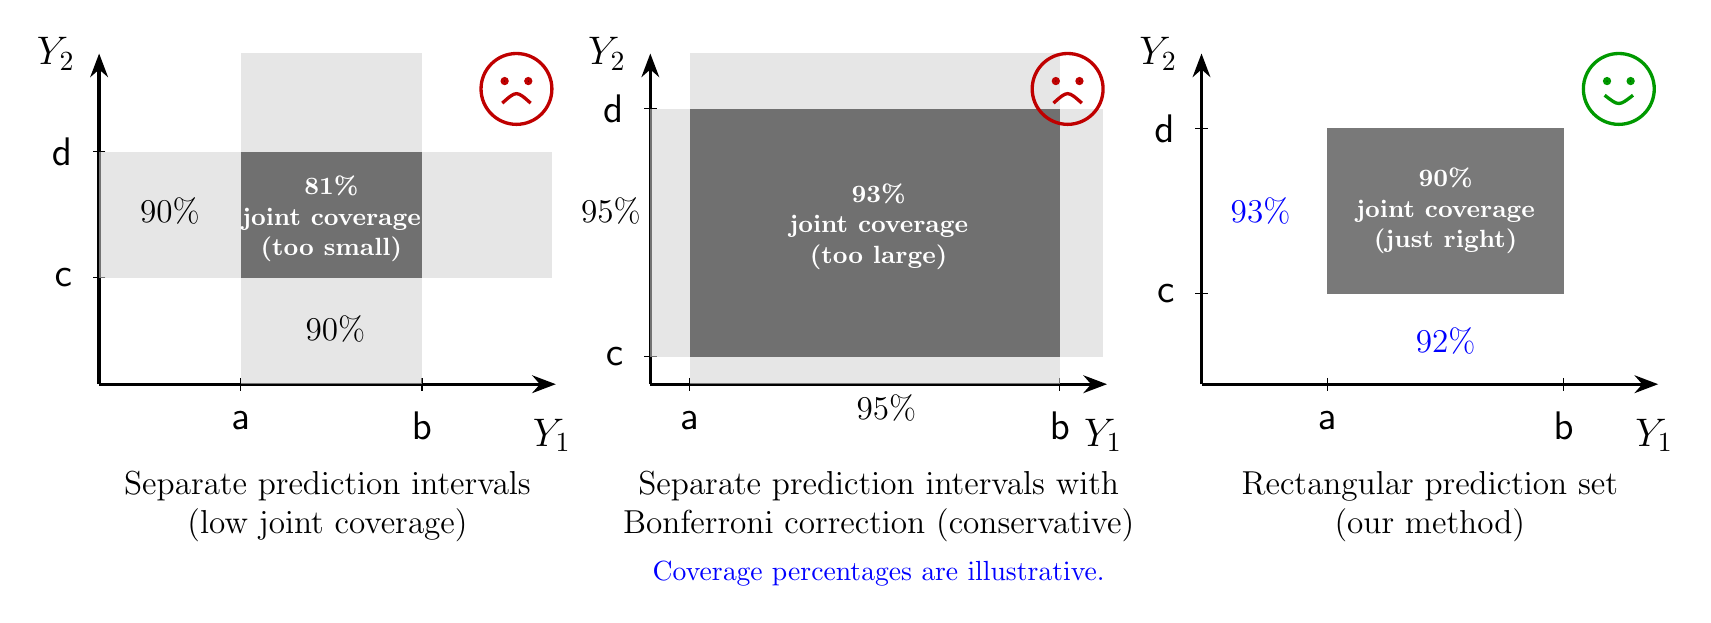
\begin{tikzpicture}[
  font=\sffamily,
  axis/.style={very thick, -{Stealth[length=3mm]}},
  tick/.style={thin},
  lightbox/.style={fill=gray!35, draw=none, opacity=0.55},
  darkbox/.style={fill=gray!60!black, draw=none, opacity=0.75},
  blob/.style={fill=gray!55!black, draw=none, opacity=0.75},
  paneltitle/.style={font=\large, align=center},
  neutral/.style={draw=orange!90!black, line width=1.2pt},
  happy/.style  ={draw=green!60!black,  line width=1.2pt},
  sad/.style    ={draw=red!75!black,    line width=1.2pt}
]

% ---------- smileys ----------
% ---------- SAD ----------
\newcommand{\placeFaceSad}[2]{% #1 = base coord, #2 = offset
  \begin{scope}
    \coordinate (FaceC) at ($(#1) + #2$);
    \draw[sad] (FaceC) circle [radius=0.45];
    \fill[sad] ($(FaceC)+(-0.15,0.10)$) circle [radius=0.03];
    \fill[sad] ($(FaceC)+( 0.15,0.10)$) circle [radius=0.03];
    \draw[sad]
      ($(FaceC)+(-0.18,-0.18)$)
      .. controls ($(FaceC)+(0,-0.02)$)
      .. ($(FaceC)+(0.18,-0.18)$);
  \end{scope}
}

% ---------- NEUTRAL ----------
\newcommand{\placeFaceNeutral}[2]{% #1 = base coord, #2 = offset
  \begin{scope}
    \coordinate (FaceC) at ($(#1) + #2$);
    \draw[neutral] (FaceC) circle [radius=0.45];
    \fill[neutral] ($(FaceC)+(-0.15,0.10)$) circle [radius=0.03];
    \fill[neutral] ($(FaceC)+( 0.15,0.10)$) circle [radius=0.03];
    \draw[neutral]
      ($(FaceC)+(-0.18,-0.12)$) -- ($(FaceC)+(0.18,-0.12)$);
  \end{scope}
}

% ---------- HAPPY ----------
\newcommand{\placeFaceHappy}[2]{% #1 = base coord, #2 = offset
  \begin{scope}
    \coordinate (FaceC) at ($(#1) + #2$);
    \draw[happy] (FaceC) circle [radius=0.45];
    \fill[happy] ($(FaceC)+(-0.15,0.10)$) circle [radius=0.03];
    \fill[happy] ($(FaceC)+( 0.15,0.10)$) circle [radius=0.03];
    \draw[happy]
      ($(FaceC)+(-0.18,-0.08)$)
      .. controls ($(FaceC)+(0,-0.22)$)
      .. ($(FaceC)+(0.18,-0.08)$);
  \end{scope}
}

% Panel geometry
\def\W{5.8}
\def\H{4.2}
\def\gap{1.2}

% =========================================================
% PANEL 1
% =========================================================
\begin{scope}[shift={(0,0)}]
  \draw[axis] (0,0) -- (0,\H);
  \draw[axis] (0,0) -- (\W,0);
  \node[rotate=0] at (-0.55,4.2) {\Large $Y_2$};
  \node at (5.75,-0.65) {\Large $Y_1$};

  \draw[tick] (1.8,0.08) -- (1.8,-0.08) node[below=4pt] {\Large a};
  \draw[tick] (4.1,0.08) -- (4.1,-0.08) node[below=4pt] {\Large b};
  \draw[tick] (0.08,1.35) -- (-0.08,1.35) node[left=4pt] {\Large c};
  \draw[tick] (0.08,2.95) -- (-0.08,2.95) node[left=4pt] {\Large d};

%  \path[lightbox] (2.35,0.55) rectangle (3.65,2.95);
  \path[lightbox]  (0,2.95) rectangle (5.75,1.35);
  \path[lightbox]  (1.8,0) rectangle (4.1,4.2);
  \path[darkbox] (1.8,1.35) rectangle (4.1,2.95);

  \node[font=\large] at (0.9,2.2) {90\%};
  \node[font=\large] at (3.0,0.7) {90\%};
  \node[align=center, font=\bfseries\small, text=white] at (2.95,2.1) {81\%\\joint coverage\\(too small)};

  % define the panel's top-right corner
  \coordinate (TR) at (\W,\H);
  % place sad face slightly inside from the top-right corner
  \placeFaceSad{TR}{(-0.5,-0.45)}


  \node[paneltitle] at (\W/2,-1.55)
    {Separate prediction intervals\\(low joint coverage)};
\end{scope}

% =========================================================
% PANEL 2
% =========================================================
\begin{scope}[shift={(\W+\gap,0)}]
  \draw[axis] (0,0) -- (0,\H);
  \draw[axis] (0,0) -- (\W,0);
  \node[rotate=0] at (-0.55,4.2) {\Large $Y_2$};
  \node at (5.75,-0.65) {\Large $Y_1$};

  \draw[tick] (0.5,0.08) -- (0.5,-0.08) node[below=4pt] {\Large a};
  \draw[tick] (5.2,0.08) -- (5.2,-0.08) node[below=4pt] {\Large b};
  \draw[tick] (0.08,0.35) -- (-0.08,0.35) node[left=4pt] {\Large c};
  \draw[tick] (0.08,3.5) -- (-0.08,3.5) node[left=4pt] {\Large d};

%  \path[lightbox] (2.35,0.55) rectangle (3.65,2.95);
  \path[lightbox]  (0,3.5) rectangle (5.75,0.35);
  \path[lightbox]  (0.5,0) rectangle (5.2,4.2);
  \path[darkbox] (0.5,0.35) rectangle (5.2,3.5);

  \node[font=\large] at (-0.5,2.2) {95\%};
  \node[font=\large] at (3.0,-0.3) {95\%};

  \node[align=center, font=\bfseries\small, text=white] at (2.9,2.0) {93\%\\joint coverage\\(too large)};

  % define the panel's top-right corner
  \coordinate (TR) at (\W,\H);
  % place sad face slightly inside from the top-right corner
  \placeFaceSad{TR}{(-0.5,-0.45)}


  \node[paneltitle] at (\W/2,-1.55)
    {Separate prediction intervals with\\ Bonferroni correction (conservative)};
\end{scope}

% =========================================================
% PANEL 3
% =========================================================
\begin{scope}[shift={(2*\W+2*\gap,0)}]
  \draw[axis] (0,0) -- (0,\H);
  \draw[axis] (0,0) -- (\W,0);
  \node[rotate=0] at (-0.55,4.2) {\Large $Y_2$};
  \node at (5.75,-0.65) {\Large $Y_1$};

  \draw[tick] (1.6,0.08) -- (1.6,-0.08) node[below=4pt] {\Large a};
  \draw[tick] (4.6,0.08) -- (4.6,-0.08) node[below=4pt] {\Large b};
  \draw[tick] (0.08,1.15) -- (-0.08,1.15) node[left=4pt] {\Large c};
  \draw[tick] (0.08,3.25) -- (-0.08,3.25) node[left=4pt] {\Large d};

  \path[darkbox] (1.6,1.15) rectangle (4.6,3.25);

  \node[align=center, font=\bfseries\small, text=white] at (3.1,2.2) {90\%\\joint coverage\\(just right)};

% BEGIN SCHEMATIC ANNOTATION R2m1
  % Illustrative probabilities: both .90, Y1 only .02, Y2 only .03, neither .05.
  \node[font=\large, text=blue] at (3.1,0.55) {92\%};
  \node[font=\large, text=blue] at (0.75,2.2) {93\%};
% END SCHEMATIC ANNOTATION R2m1
    \coordinate (TR) at (\W,\H);
    \placeFaceHappy{TR}{(-0.5,-0.45)}     % panel 3


  \node[paneltitle] at (\W/2,-1.55)
    {Rectangular prediction set\\(our method)};
\end{scope}

% BEGIN SCHEMATIC ANNOTATION R2m1
\node[font=\normalsize, text=blue] at (\W+\gap+\W/2,-2.4)
  {Coverage percentages are illustrative.};
% END SCHEMATIC ANNOTATION R2m1
\end{tikzpicture}
\end{document}

%%% Local Variables:
%%% mode: latex
%%% TeX-master: t
%%% End:
